
\chapter{Disk and File}


\section{Introducing Disk Topology}




\highlightdef{A \textbf{Cylinder} is a collection of tracks 
with the \textit{same radius} but on \textit{different platters}}

Each cylinder is determined by its radius $r$. 
Assuming the \textit{virtual geometry} can assume that each cylinder 
has the same number of tracks. 
We will use the notation \textsc{c}[$r$] to denote a cylinder 
(the vertical stack of tracks) that are at radius $r$. 


The \textsc{os} treats the hard disk as a one-dimensional array of \textit{disk blocks}.

\highlightdef{The \textbf{Disk Block Size} is a \textit{convenient} 
fixed \textit{byte size} chosen by the \textsc{os}}

The point of this definition is defining 
what it means to have a block size that is \textit{convenient}.
Designing data structutes to work on the byte-level (or bit-level) is too complicated. 
And, the chances are, the structure will be too inefficient.

\highlightdef{\textbf{Logical block addressing} is a simple linear addressing scheme 
where blocks are uniquely addressed by an integer index}

\begin{example}
The \textsc{ide} standard included 22-bit LBA option. 
Howw many disk blocks can be addressed under these scheme?
\end{example}


\frmrule

Assuming we only need \textit{one track} for disk transfer and 
request to read/write $b$ \textit{contiguous} bytes on that track, then
a request to read and writing disk blocks can be done in three steps. 

\begin{itemize}   
\renewcommand{\labelitemi}{$\Box$}
\item \textbf{Seek}
We move the radius of the read/write heads to change the current cylinder.
This changing of radius is called \textit{seeking}. Once we reach the 
radius/cylinder with the track we need, we stop seeking.
The time it takes for read/write heads to change to the required radius is 
called the \textit{seek time}.
\item \textbf{Wait}
Next, we wait for the disk to rotate so that the first sector is under the head.
The time we wait for the disk to rotate in this step is referred to as 
\textit{rotational latency}.
\item \textbf{Transfer}
Now that the head is finally positioned correctly, we begin the transfer 
(reading or writing). Under our assumption, we read/write contiguous blocks 
and on only on a single track.
The time spend transferring data from the track to the disk controller
is called the \textit{transfer time}.
\end{itemize}

We also assume that the \textit{spinup time} 
(time for platters to start to accelerate to constant angular velocity from rest).
For this three-step model, the average time is given by:

\highlightdef{The \textbf{Average Turnaround Time} is
$T = t_{\text{seek}} + \frac{1}{2}  \frac{1}{r} + \frac{b}{N} \frac{1}{r}$
}

in seconds, where $t_{\text{seek}}$ is the cylinder seek time,
$b$ is how many bytes in the request, $N$ is the number of bytes in each track, 
$r$ is the rotational frequency (the number revolutions per second).

Note that $\frac{1}{r}$ is the total time it takes for the disk to complete one revolution. 
In the worst case, we wait $\frac{1}{r}$ seconds for the disk to rotate a full revolution 
because we just missed it. In the best case, the disk is at the perfect position and we 
wait 0 seconds. The time it takes is a uniform random variable. So the \textit{average} time 
it takes for the disk to rotate to where we need it is  
$\frac{1}{2} \times \frac{1}{r}$. This is the \textit{average rotational latency}. 

As we are reading/writing, the disk is still rotating. 
The more bytes we read, the more longer the rotation time we 
need. The fraction $\frac{b}{N}$ is \textit{what fraction of the track} we need for 
reading/writing. Here, $0 \leqslant b \leqslant N$. If we read/write the whole track, $b = N$, 
if we read/write to none of it $b = 0$, and if we 
read/write, say, a contiguous 30 percent of the track, then $\frac{b}{N} = 0.3$. 
The overall time for doing reading/writing is the \textit{fraction of the track we need} 
for the reading/writing multiplied by \textit{the total time to go around the track}.
This is the \textit{transfer time} of $\frac{b}{N} \times \frac{1}{r}$. 

\frmrule

\begin{tikzpicture}
  % disk
  \draw[black!20] (0cm,0cm) circle(0.3cm);
  \draw[black!20, very thick] (0cm,0cm) circle(1.2cm);
  \draw[black!20] (0cm,0cm) circle(2.5cm);
  \foreach \x in {0,5,...,360} {
    \draw[dashed,black!20] (\x:0.3cm) -- (\x:2.5cm);
  }
  % transfer time arc with label
  \draw [|-|, thick] (0cm,0cm) ++(30:1.2cm) arc (30:300:1.2cm);
  \node at (180:2.2cm) (seek) {transfer};
  \coordinate (seekfr) at ($(seek)+(0.0cm,-0.4cm)$);
  \node at (seekfr) {$\frac{b}{N} = 0.75$};
  % seek time with label
  \draw [<-, dashed] (340:1.25cm) -- (340:2.0cm);
  \draw (340:2.5cm) node (seek) {seek};
  % rotational latency arc with label
  \draw [<->, dashed] (0cm,0cm) ++(300:1.2cm) arc (300:340:1.2cm);
  \draw (320:1.6cm) node {wait};



\end{tikzpicture}

\frmrule

\begin{example}
Explain why we cannot have $b > N$.
\end{example}

\begin{example}
Do we need to know whether the disk is rotating clockwise or anticlockwise to use 
the turnaround time equation? Explain your answer.
\end{example}

\begin{example}
How many revolutions does the disk complete while the head is seeking?
\end{example}




\frmrule

\highlightdef{The \textbf{Cylinder Seek Time} affects the turnaround time \textit{greatly} }

To improve disk performance, a hard disk driver therefore attempts
to control how the head moves in an attempt to give the smallest seek time. 
The concept of controlling head's radius according to \textsc{io} requests is called 
\textit{cylinder seek scheduling}. There have been several \textit{scheduling algorithms} 
developed that attempt to give the smallest seek time and can significantly reduce 
the turnaround time.  



\begin{figure}[h]
\begin{tikzpicture} [
  every node/.style={node_sty, align=center},
  edge from parent/.style={edge_sty},
  edge from parent path={(\tikzparentnode.south) 
   |- ($(\tikzparentnode.south)!0.5!(\tikzchildnode.north)$) -| (\tikzchildnode.north)},
  level 1/.style={sibling distance=2cm, level distance = 0.9cm},
  ro/.style={text width=5cm},
  ch/.style={text width=1.4cm},
]
  \node [ro]
  (root) {Cylinder Seek Scheduling}
    child {node[ch] (pio) {FCFS}}
    child {node[ch] (intio) {SSTF}}
    child {node[ch] (intio) {SCAN}}
    child {node[ch] (intio) {CSCAN}}
    child {node[ch] (intio) {NSCAN}};
   
\end{tikzpicture}
\end{figure}

\begin{itemize}   
\renewcommand{\labelitemi}{$\Box$}
\item \textbf{FCFS} 
This is short for \textit{First Come First Served}. 
We seek to the cylinders in the order the requests arrived. 
\item \textbf{SSTF}
This is short for \textit{Shortest Seek Time First}. 
We seek to the cylinder that is closest (shortest difference in radius) 
to the current radius of the disk heads. 
\item \textbf{SCAN}
We \textit{temporarily maintain a fixed direction} while processing requests. 
When there are no requests left in the fixed direction, we change direction and 
temporarily maintain that direction. 
We always process requests that are the closest to current radius of the disk heads. 
\item \textbf{CSCAN}
This is called \textit{continuous} \textsc{scan}. 
We \textit{continuously maintain a fixed direction} while processing requests.
When there are no requests left in our fixed direction,
we change direction \textit{once} to go to the request that's furthest away, 
but then resume processing requests in our fixed direction. 
\item \textbf{NSCAN}
This is called \textit{n-step} \textsc{scan}. This is a modification to \textsc{scan}.
When we begin/change direction we remember these requests at this point in time and only
process those. If any new requests that arrive, they will only be 
considered at the next direction change. 
\end{itemize}

To get a more concrete understanding of these algorithms, let's look at some examples.

\frmrule

\begin{example}
Below shows an example of FCFS with the queue: 98, 183, 37, 122, 14, 130, 60, 67
with initial head position $h_0 = 53$. 

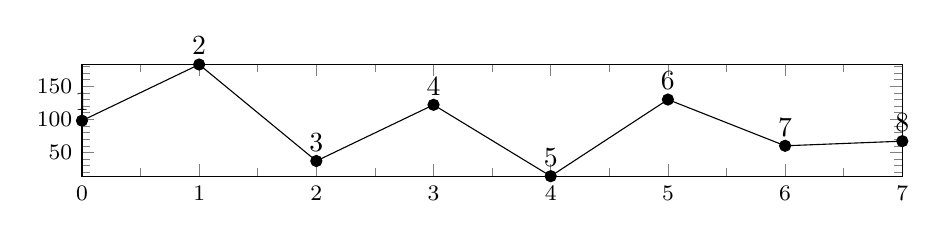
\begin{tikzpicture}
\pgfplotsset{width=12cm, height=3cm}
\selectcolormodel{gray}
\begin{axis}[
  enlargelimits=false, 
  tick label style={font=\footnotesize},
  minor x tick num=1,
  minor y tick num=4
]
  \addplot[sharp plot, mark=*, nodes near coords, point meta=explicit symbolic] coordinates
  {(0,98)[1] (1,183)[2] (2,37)[3] (3,122)[4] (4,14)[5] (5,130)[6] (6,60)[7] (7,67)[8]};

\end{axis}
\end{tikzpicture}
\end{example}

\frmrule

\begin{example}
Below shows an example of SSTF with the queue: 98, 183, 37, 122, 14, 130, 60, 67
with initial head position $h_0 = 53$. 

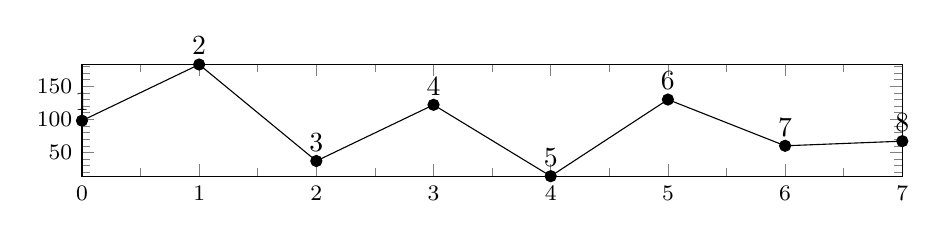
\begin{tikzpicture}
\pgfplotsset{width=12cm, height=3cm}
\selectcolormodel{gray}
\begin{axis}[
  enlargelimits=false, 
  tick label style={font=\footnotesize},
  minor x tick num=1,
  minor y tick num=4
]
  \addplot[sharp plot, mark=*, nodes near coords, point meta=explicit symbolic] coordinates
  {(0,98)[1] (1,183)[2] (2,37)[3] (3,122)[4] (4,14)[5] (5,130)[6] (6,60)[7] (7,67)[8]};

\end{axis}
\end{tikzpicture}
\end{example}

\frmrule

\begin{example}
Below shows an example of SCAN with the queue: 125, 95, 33, 174, 8, 19, 58, 79, 195
with initial head position $h_0 = 100$ and initial direction of +. 

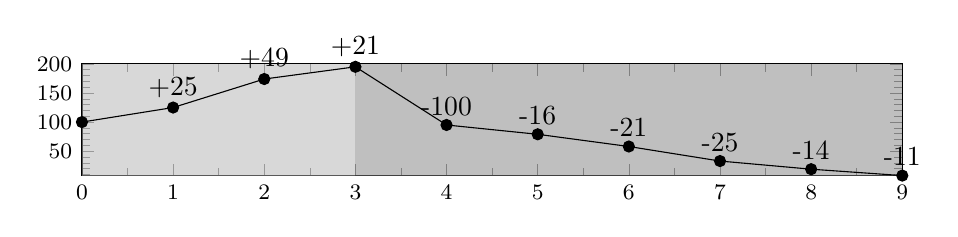
\begin{tikzpicture}
\pgfplotsset{width=12cm, height=3cm}
\selectcolormodel{gray}
\begin{axis}[
  enlargelimits=false, 
  tick label style={font=\footnotesize},
  minor x tick num=1,
  minor y tick num=4
]
  \addplot[draw=none, area style, fill=black!30, opacity=0.5] coordinates
  {(0,200) (3,200)}\closedcycle;
  \addplot[draw=none, area style, fill=black!50, opacity=0.5] coordinates
  {(3,200) (9,200)}\closedcycle;

  \addplot[sharp plot, mark=*, nodes near coords, point meta=explicit symbolic] coordinates
  {(0,100) (1,125)[+25] (2,174)[+49] (3,195)[+21] (4,95)[-100] (5,79)[-16] (6,58)[-21] (7,33)[-25] (8,19)[-14] (9,8)[-11]};

\end{axis}
\end{tikzpicture}
\end{example}




\frmrule

Below shows an example of how we might write pseudocode for the scheduling algorithms.


\section{File Allocation Tables}

Associate with each disk exactly one table 
called the \textit{file allocation table}, \textsc{fat}.
This is a table that stores information about \textit{every disk block}. 
We will write \textsc{fat}[$k$] to denote the information the table has on the $k$th block.

Each file is uniquely associated with its first block
on disk, e.g. first(F) = 8 means that the first block
of file F is disk block no8.
• FAT[k] denotes the next disk block of the file whose
data is also stored on disk block nok.
If FAT[k] = EOF then disk block nok was the file’slast block.
FAT[k]= FREE denotes an unused block; FAT[k]=
BAD denotes a bad block, etc.


\section{UNIX Fast File System}

Original \textsc{unix} File System (\textsc{ufs}).
Simple, elegant, but \textit{slow}.


Each file is described by an \textit{index node}.
Index nodes are data structures used to store information about each file
An \textit{inode} may contain references to single, double 
and triple indirect blocks.

An \textit{inode number} uniquely identifies an inode.
There is precisely one inode per file that acts as a root.

\highlightdef{An \textbf{index node} (inode) is the root of a tree of references to 
the blocks of a file}.

An \textit{inode} can be in two locations:




\begin{lstlisting}
typedef struct{
unsigned inode_number : 16; /* 2 bytes */
char file_name[14] : 112; /* 14 bytes */
} DIRECTORY_ENTRY
\end{lstlisting}




\begin{example}
For a particular filesystem, an inode contains 8 direct pointers, 
1 pointer to an indirection block and 1 pointer to a 
two-level indirection block. 
Each pointer is $p$ bytes. Each disk block is $b$ bytes.
Each indirection block has $k$ pointers.

For this file system, \\
(a) determine the maximum file size \\
(b) determine the disk space required to store this file
\end{example}

\frameans{}{
	(a) $(8+k+k^2)b$ \\
	(b) $(8+k+k^2)b + (10+2k+k^2)p$
}

Drawing a diagram is useful for this question. 

\begin{tikzpicture}[
      start chain=1 going right,
      start chain=2 going right,
      node distance=0mm,
      inode/.style={draw, minimum height=1.4em,
      text width=2em, text centered, inner sep=1.7pt}
  ]
  % Index node
  \node[on chain=1, inode, text width=6em] (i1) {$8p$};
  \node[on chain=1, inode] (i2) {$p$};
  \node[on chain=1, inode] (i3) {$p$};
  % Data nodes
  \node[inode, below=2.1cm of i2] (d1) {$kp$};
  \node[inode, below=0.8cm of i3] (d2) {$kp$};
  \node[inode, below=0.8cm of d2] (d3) {$kp$};
  % File nodes
  \node[on chain=2, below=1cm of d3, inode, text width=2em, xshift=-3cm] (f1) {$b$};
  \node[on chain=2, inode, text width=5em] (f2) {$b$};
  \node[on chain=2, inode, text width=8em] (f3) {$b$};

  % Draw edges and the slashes/ticks on edges
  
  \draw [->] (i1) |- node[pos=0.25, name=s1, rotate=70] {\tiny$/$} ($(f1)+(0.0cm, 0.5cm)$) -- (f1);
  \draw [->] (i2) -- node[pos=0.25, name=s2, rotate=70] {\tiny$/$} (d1);
  \draw [->] (i3) -- node[pos=0.5, name=s3, rotate=70] {\tiny$/$} (d2);
  \draw [->] (d2) -- node[pos=0.5,name=s4, rotate=70] {\tiny$/$} (d3);
  
  \draw [->] (d1) |- node[pos=0.3, name=s5, rotate=70] {\tiny$/$} ($(f2)+(0.0cm, 0.5cm)$) -- (f2);
  
  \draw [->] (d3) |- node[pos=0.7, name=s6, rotate=70] {\tiny$/$} ($(f3)+(0.0cm, 0.5cm)$) -- (f3);

  \node[left=0.05cm of s1, yshift=0.2cm] {8};
  \node[left=0.05cm of s2, yshift=0.2cm] {1};
  \node[left=0.05cm of s3, yshift=0.2cm] {1};
  \node[left=0.05cm of s4, yshift=0.2cm] {$k$};
  \node[left=0.05cm of s5, yshift=0.2cm] {$k$};
  \node[right=0.05cm of s6, yshift=0.1cm] {$k$};

  % Background Shadows
  \begin{pgfonlayer}{background} 
  \node[fill=black!10,drop shadow,draw=none,inner sep=0pt, fit = (i1) (i3)] (background) {};
  \node[fill=black!10,drop shadow,draw=black,inner sep=2pt, fit = (f1) (f3)] (background) {};
  \end{pgfonlayer}

  % Manually draw the strike thru
  %\coordinate (m1) at ($(i1)-(0, 1.5cm)$);
  %\draw [-] ($(m1)-(0.15,0.15)$) -- ($(m1)+(0.15,0.15)$);
  %\coordinate (m2) at ($(i2)!0.5!(d1)$);
  %\draw [-] ($(m2)-(0.15,0.15)$) -- ($(m2)+(0.15,0.15)$);


  %
  %\coordinate (MidWay) at ($(2.east)!0.5!(1.west)$);
  %\draw [thick, red,-] ($(MidWay)-(0.15,0.15)$) -- ($(MidWay)+(0.15,0.15)$);

\end{tikzpicture}

From the diagram, we can work out the required values:\\
(a) The total file size is $8b + kb + k^2b = (8+k+k^2)b$ \\
(b) The total file size plus the size of the pointers which is:
$[(8+k+k^2)b] + [(8p + p + p) + (kp) + (kp) + (k^2p)] = (8+k+k^2)b + (10+2k+k^2)p$










\begin{example}
In the \textit{Linux ext2fs filesystem}, an inode has 15 pointers.
The first 12 pointers directly locate 12 data blocks, 
the 13th is an indirect pointer, the 14th is a doubly-indirect pointer and the 
15th is triply-indirect pointer. 

Each of these pointers is 8 bytes long.

\end{example}


\section{Disk Caching}



\section{UNIX Block Buffer Cache}

We can cache files in main memory for a speedup (compared to accessing the files 
from disk). The cache works in the usual manner, we have a cache hit case and a 
cache miss case.



\section{UNIX inodes}




\section{Virtual File Systems}


\section{UNIX Permissions}


\highlightdef{\textsc{unix} has access levels: 
\textbf{r} for \textit{read},
\textbf{w} for \textit{write},
\textbf{x} for \textit{execution}}

\highlightdef{\textbf{Symbolic notation} is a sequence of 
9 binary flags where the \textit{symbol} 
(either \lstinline{r},\lstinline{w}, or \lstinline{x})
is written for 1, and a \textit{dash} (\lstinline{-}) is written for 0}

\begin{example}
Write the flags 001100011 in symbolic notation.

We replace the zeros with \lstinline{-} and replace the ones with the 
appropriate symbol based on their position 
(following the pattern \textit{rwx,rwx,rwx}). 
The \textit{symbolic notation} is therefore: \lstinline{--xr---wx}

\end{example}

\frmrule


Note that \textit{three binary digits} corresponds exactly with one \textit{octal digit}. 
As a result, the symbol notation corresponds to 9 binary digits or 3 octal digits. 
The \textit{octal notation} gives a sequence of octal digits that correspond to the 
9 binary flags. 

\frmrule

\begin{example}
Write the flags 001100011 in octal notation.

The first three digits, 001, correspond to octal digit 1. \\
The next three digits, 100, correspond to octal digit 4. \\
The last three digits, 011, correspond to octal digit 3. \\
Hence the octal notation is: 143.
\end{example}

\begin{example}
Give the symbolic representation that corresponds to octal notation 777.
\end{example}




\section{File System Recovery}

storage devices still mess up – they have
so-called bad blocks that make it hard to keep a file
system reliable.

simply backup the system regularly so that
parts of it can be restored when a bad block occurs.
The problem is how to do backups efficiently:

incremental dumps, by which changes are added
to the backup, say, every day
use doubling technique, such as doing writes to
two drives, but reading only from one.




\section{\textsc{raid} Storage}

Properties of XOR: